
%\documentclass[12pt,notitlepage,aps,pra,longbibliography,nofootinbib,tightenlines]{revtex4}
\documentclass[12pt,notitlepage,longbibliography,nofootinbib,tightenlines]{revtex4-1}

%\documentclass[12pt,a4]{revtex4}
%\documentclass[12pt]{article}
%\documentclass[11pt, twocolumn]{article}

%\usepackage{epsf}
\usepackage{amsmath}
\usepackage{color}
\usepackage{natbib}
%\usepackage{cite}

\RequirePackage{amsmath}
\RequirePackage{amssymb}
\RequirePackage{amsthm}
%\RequirePackage{algorithmic}
%\RequirePackage{algorithm}
%\RequirePackage{theorem}
%\RequirePackage{eucal}
\RequirePackage{color}
\RequirePackage{url}
\RequirePackage{mdwlist}

\RequirePackage[all]{xy}
\CompileMatrices
\RequirePackage{hyperref}
\RequirePackage{graphicx}
%\RequirePackage[dvips]{geometry}


\begin{document}

%\title{Representations of Pauli Operator Hamiltonians}
\title{Representations of Subsystem Code Hamiltonians}

\author{Simon Burton}
\affiliation{Centre for Engineered Quantum Systems, School of Physics, The University of Sydney}

\date{\today}

%\begin{abstract}
%The Pauli algebra terms used in a Hamiltonian
%carry a multiplicative group structure echoing
%the action of the Hamiltonian on states.
%The representation theory of this group
%shows how to decompose the action into
%invariant sub-actions, which corresponds
%to block diagonalizing the Hamiltonian.
%\end{abstract}

\begin{abstract}
We analyse the (multiplicative) group structure of terms arrising
in Hamiltonians constructed from Pauli operators.
We decompose these operators into irreducible 
representations, which corresponds to block diagonalizing
the Hamiltonian where the blocks are labelled by
eigenvalues of integrals of motion.
We apply this technique to the 2d-compass model
and the Kitaev honeycomb model.
%and find results
%similar to those previously known,
%however, we use only the structure of the gauge group,
%and not any transformations at the level
%of spins. 
The results are similar to those previously 
calculated via spin transformations,
however, we perform transformations at
the level of the structure of the gauge group.
\end{abstract}

\maketitle


\def\Complex{\mathbb{C}}
\def\Z{\mathbb{Z}}
\def\Ham{\mathcal{H}}
\def\Pauli{\mathcal{P}}
\def\Spec{\mbox{Spec}}
\def\Proveit{{\it (Proof??)}}
\def\GL{\mathrm{GL}}
\def\half{\frac{1}{2}}
\def\Stab{S}


%%%%%%%%%%%%%%%%%%%%%%%%%%%%%%%%%%%%%%%%%%%%%%%%%%%%%%%%%%%%%%%%%%%%%%%%%%%%%%%
%
%%%%%%%%%%%%%%%%%%%%%%%%%%%%%%%%%%%%%%%%%%%%%%%%%%%%%%%%%%%%%%%%%%%%%%%%%%%%%%%
%

%\section{Introduction}

%Transverse field Ising model:
%$$
%    \Ham = \sum_i X_i X_{i+1} + Z_i.
%$$
%The $XY$ model:
%$$
%    \Ham = \sum_i X_i X_{i+1} + Z_i Z_{i+1}.
%$$
%In both these cases the existence of large weight stabilizer generators
%causes the gapless behaviour.

Quantum error correcting codes,
in particular {\it stabilizer codes} \cite{Gottesman1997},
aim to protect an encoded quantum state
by measuring a collection of commuting
observables.
When these same observables are used as
the terms of a Hamiltonian 
a dynamical picture emerges: the
encoded state now belongs to the
(degenerate) groundspace of a
system \cite{Dennis2001}. 
Questions about protecting
this state are now related to questions about
the spectrum of this Hamiltonian.

A more general notion of error correction
comes from the theory of 
{\it subsystem} codes \cite{Poulin2005}. 
Here the observables
no longer commute, which complicates
the error correction procedure.
Also, the corresponding Hamiltonian
has non-commuting terms, but
we may still find integrals of
motion that label eigenspaces
of the system.

We elucidate these ideas using representation theory. 
The group generated by the terms of the Hamiltonian
will be called the {\it gauge group},
and the intuition is that this
group acts on itself in much the same way
that it acts on states. 
Indeed, we forget all about the state space and
examine the structure of the group itself.

When this approach succeeds we find we can
block diagonalize Hamiltonian made from 
the Pauli spin operators
$I$ $X$ $Z$ and $Y$, with coupling coefficients
$\pm 1.$
The blocks are labelled by eigenvalues of
integrals of motion generated by the gauge
group. These operators are the {\it stabilizers.}
For Hamiltonians such as
the transverse-field Ising model,
$\Ham = \sum_i X_i X_{i+1} + Z_i,$
this is not much use because the 
gauge group does not generate many
stabilizers (in fact, only one in this case).
We are more interested in the situation
where the gauge operators generate a large 
number of stabilizers, and we examine two
such cases: the 2d-compass model \cite{Bacon2006} and
the Kitaev honeycomb model \cite{Kitaev2006}.

%refs to cite:
%http://arxiv.org/pdf/0908.4246.pdf
%http://arxiv.org/pdf/1207.1443.pdf
%http://arxiv.org/abs/0907.0948
%http://arxiv.org/pdf/1008.1029v1.pdf
%http://arxiv.org/abs/1107.2707
%http://arxiv.org/pdf/1012.0425v2.pdf


%    %The quantum error correcting codes,
%    %in particular {\it stabilizer codes},
%    provide a way of building Hamiltonians
%    with many integrals of motion.
%    When all terms commute,
%    these terms are called stabilizers
%    because they do not effect the groundstate.
%    %Other commuting operators, outside of the stabilizer
%    %group are called logical operators because
%    %they change the groundstate.
%    We can simultaneously diagonalize each
%    term in such a Hamiltonian, and so label
%    eigenvectors by the eigenvalue of each
%    stabilizer.
%    The stabilizer group is the group generated
%    by these Hamiltonian terms.
%    
%    More generally, {\it subsystem codes} protect an
%    encoded state via measurement of non-commuting
%    operators, called gauge operators.
%    Hamiltonians build from these operators 
%    once again aim to protect the encoded state
%    energetically, but now we cannot solve (diagonalize)
%    such a system so easily.
%    However, we do still find integrals of motion:
%    these stabilizers are now {\it generated} by gauge operators,
%    and commute with each of these gauge operators.
%    
%    Other operators build from the entire $n$-qubit Pauli
%    group that commute with the Hamiltonian therefore
%    act on the degenerate eigenspaces, and are called
%    {\it logical operators}.
%    
%    %and other operators (logical operators)
%    %that commute with every
%    %term and so act on the degenerate eigenspaces.
%    
%    Stabilizer codes, and more generally, subsystem codes
%    \cite{Poulin2005}, \cite{Bacon2006}
%    attempt to store quantum information using
%    an error correction proceedure...
%    group structure of the measurement operators
%    that allows to prove some nice properties of the
%    error correction proceedure.
%    
%    A dynamical picture emerges when we consider a
%    Hamiltonian built from the sum of these exact same
%    operators (up to a sign).
%    Now the encoded information is stored in the
%    groundspace of a degenerate Hamiltonian.
%    Now we ask if the energetics of the system
%    has any robustness to excitations..
%    in particular the low energy spectrum,
%    can maintain ..
%    
%    from the coding point of view, distance matters
%    as well as number of encoded qubits. subsystem codes
%    also would need bounded gauge operators per stabilizer
%    in order to be fault tolerant (or have error threshold)
%    
%    from the dynamical point of view, the first (of many)
%    questions to ask is: does the spectrum have a gap?
%    Also, this is perhaps a wider class of systems, as we
%    may be interested in Hamiltonians with non-degenerate 
%    groundstate
%    (thought of as a code these systems do not store any information.)
%    
%    The usual way of attacking these Hamiltonians is
%    by doing some kind of ad-hoc spin transformation.
%    Here we show a method that is one level
%    above such transformations of the hilbert space:
%    we transform the (group of) operators themselves.
%    % drawback of complicating the analysis of Hamiltonians
%    % with J's.
%    
%    We are interested in diagonalizing (solving) Hamiltonians
%    built from Pauli operators, whose terms are not necessarily commuting.
%    An example of this is the 
%    transverse-field Ising model:
%    $\Ham = \sum_i X_i X_{i+1} + Z_i.$
%    The usual way of attacking these Hamiltonians is
%    by doing some kind of ad-hoc spin transformation.
%    Here we show that the group structure of the 
%    Hamiltonian terms reveals similar transforms,
%    in a simpler and more general way.
%    We apply these group theory techniques
%    to the 2D-compass model and the Kitaev honeycomb
%    model.

%\section{Representations of gauge codes}

%It follows that the adjacency matrix $A$ of Cayley($G$, $G_0$)
%is the linear operator $A:\Complex[G]\to\Complex[G]$
%given by
%$$
%    A = \sum_{g\in G}\alpha(g) \rho_{\mathrm{reg}}(g)
%$$
%where $\rho_{\mathrm{reg}}$ is the left regular representation of
%$G$ on $\Complex[G],$
%and the indicator function $\alpha:G\to\Complex$ is
%$$
%    \alpha(g) := \left\{ \begin{array}{ll}
%1 &\mbox{if $g\in G_0$; and}\\
%0 &\mbox{otherwise.}\end{array} \right.
%$$
%
%Given a group representation $\rho:G\to \mathrm{GL}(V)$,
%and function $\phi:G\to \Complex,$
%the {\it Fourier transform} % of $\phi$ relative to $\rho$,
%$\hat\rho(\phi)\in \mathrm{GL}(V)$ is defined as
%$$\hat\rho(\phi) := \sum_{g\in G} \phi(g)\rho(g).$$
%
%Then we have
%$$
%    \hat\rho(\alpha) = \sum_{g\in G_0} \rho(g).
%$$
%
%\noindent{\bf Theorem.} 
%(See \cite{Kaski2002} and \cite{Diaconis1981})
%The spectrum of the adjacency matrix $A$ of a
%cayley graph Cayley($G$, $G_0$) equals the union
%of the spectra of fourier transforms of the indicator
%function $\alpha$ of the generating set $G_0$:
%$$
%    \Spec(A) = \bigcup_{\mathrm{irrep}\ \rho} \Spec(\hat\rho(\alpha))
%$$

%%%%%%%%%%%%%%%%%%%%%%%%%%%%%%%%%%%%%%%%%%%%%%%%%%%%%%%%%%%%%%%%%%%%%%%%%%%%%%%
%
%%%%%%%%%%%%%%%%%%%%%%%%%%%%%%%%%%%%%%%%%%%%%%%%%%%%%%%%%%%%%%%%%%%%%%%%%%%%%%%
%

\subsection{Motivation: graph theory}

\begin{figure*}[th!]
\begin{center}
        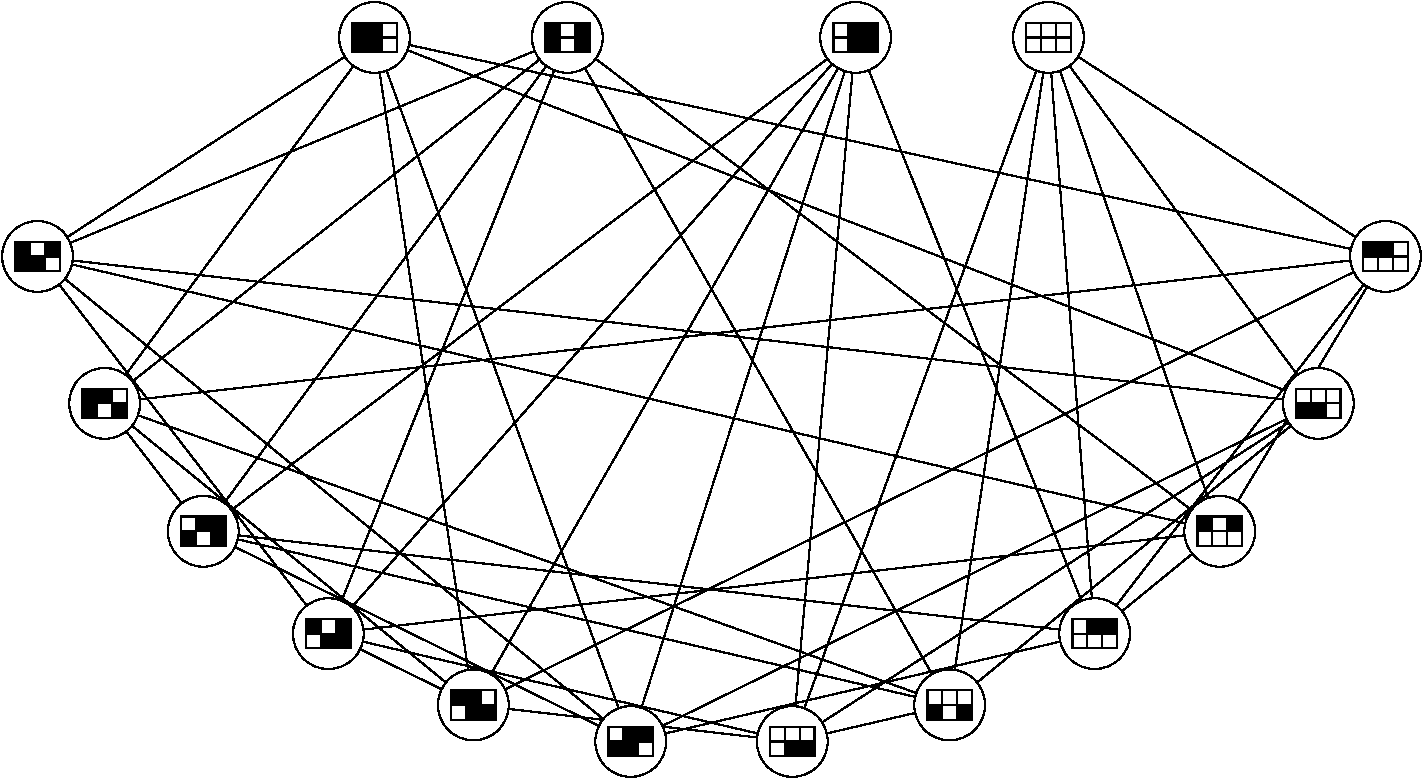
\includegraphics[width=0.9\columnwidth]{fig_compass.pdf}
\caption{
The gauge group action on a basis is depicted as a graph.
}
\label{fig_compass}
\end{center}
\end{figure*}

\def\rhoreg{\rho_\mathrm{reg}}

Given a group $G$ and a set $V$,
a {\it group action} 
is a function $\eta$ that associates
each $g\in G$ with a bijection $\eta(g):V\to V.$
%Given a group action $\eta$ of $G$ on a set $V$ and a
Given such a group action and a
set $G_0\subset G$ we can form a graph as
follows.
The vertices correspond to the set $V$ and
(directed) edges are  $\{(v, gv) : v \in V, g \in G_0\}.$
If the set $G_0$ is closed under group inverse then
we can consider the graph to be undirected.
The complex vector space with basis $V$ is written $\Complex[V].$
We can now extend $\eta$ linearly to get a {\it representation} of
the group $G$:
$$
    \Complex[\eta] : G \to GL(\Complex[V]).
$$

We show in Fig \ref{fig_compass} the action
of the 
the following subset of the 6-qubit Pauli group %$\Pauli_6$
on the computational basis:
$$
\arraycolsep=-1pt\def\arraystretch{0.2}
G_0 = \Bigl\{
\begin{array}{ccc}
X&X&I\\
I&I&I
\end{array},
\begin{array}{ccc}
I&I&I\\
X&X&I
\end{array},
\begin{array}{ccc}
I&X&X\\
I&I&I
\end{array},
\begin{array}{ccc}
I&I&I\\
I&X&X
\end{array},
\begin{array}{ccc}
X&I&X\\
I&I&I
\end{array},
\begin{array}{ccc}
I&I&I\\
X&I&X
\end{array},
\begin{array}{ccc}
Z&I&I\\
Z&I&I
\end{array},
\begin{array}{ccc}
I&Z&I\\
I&Z&I
\end{array},
\begin{array}{ccc}
I&I&Z\\
I&I&Z
\end{array}
\Bigr\}
$$

The {\it Cayley graph} of a group $G$ and
generating set $G_0$ is denoted Cayley($G$, $G_0$).
It has nodes $G$ and edges $\{(g, hg) : g \in G, h \in G_0\}$.
%We will always assume $G_0$ is closed under group inverse,
%and so we can consider the Cayley graph as undirected.
This is the graph associated with the group action on itself.
The group action on itself is in some sense the ``mother'' of all other ways that
$G$ can act on a set, and likewise the Cayley graph is the ``most relaxed'' version
of all graphs obtained in this way from $G$ acting on a set.

The adjacency matrix of a graph with $N$ nodes is the 
$N$ by $N$ matrix $A$ with non-zero entries $A_{ij}=1$ corresponding
to edges $(i, j)$ of the graph.
It follows that the adjacency matrix $A$ of Cayley($G$, $G_0$)
is the linear operator $A:\Complex[G]\to\Complex[G]$
given by
$$
    A = \sum_{g\in G_0}\rho_{\mathrm{reg}}(g)
$$
where $\rho_{\mathrm{reg}}$ is the left regular representation of
$G$ on $\Complex[G].$

Using representation theory we have that 
$\rhoreg:G\to \Complex[G]$
decomposes as the dirrect sum of irreducible
representations $\rho_k:G\to \GL(V_k)$
and so
$$
    A = \sum_{g\in G_0}\bigoplus_k \rho_k(g)
$$

block diagonalizes $A$,
with each $\rho_k$ possibly appearing multiple
times in the direct sum over $k$.

Given a function $f:G\to\Complex$
and a representation $\rho:G\to \GL(V)$
the \emph{Fourier transform}
of $f$ relative to $\rho$ is defined as
$$
\hat{\rho}(f) := \sum_{g\in G}f(g)\rho(g).
$$
This will be a linear operator on $V.$

See \cite{Diaconis1981} and \cite{Kaski2002} for more details.

%%%%%%%%%%%%%%%%%%%%%%%%%%%%%%%%%%%%%%%%%%%%%%%%%%%%%%%%%%%%%%%%%%%%%%%%%%%%%%%
%
%%%%%%%%%%%%%%%%%%%%%%%%%%%%%%%%%%%%%%%%%%%%%%%%%%%%%%%%%%%%%%%%%%%%%%%%%%%%%%%
%

\subsection{Representations of Gauge codes}

The Pauli group $\Pauli_1$ is normally 
defined as a set of matrices closed under
matrix multiplication, but we can define
it abstractly
as the group generated
by the (abstract) elements $\{\omega, X, Z\}$ with
relations as follows:
$$
\omega^2=I,\ X^2=I,\ Z^2=I,\ \omega X\omega X=I,\ \omega Z\omega Z=I,\ \mbox{and}\  \omega ZXZX=I,
$$
where $I$ is the group idenity.
Actually, $\omega $ is generated by $X$ and $Z$, so
it is not necessary to include $\omega $ in the generating set,
but here it simplifies the relations.

To define the $n$-qubit Pauli group $\Pauli_n$, 
we use the $2n+1$ element 
generating set $\{\omega , X_1, .., X_n, Z_1, .., Z_n\}$
with relation $\omega^2=I$ as before, and
\begin{equation}\label{presentation}
\begin{array}{c}
X_i^2=I,\ Z_i^2=I,\ \omega X_i\omega X_i=I,\ \omega Z_i\omega Z_i=I,\ \omega Z_iX_iZ_iX_i=I, 
\mbox{\ for\ } i=1,...n,\\
Z_iX_jZ_iX_j=I, \mbox{\ for\ } i, j = 1,..,n,\ i\ne j.
\end{array}
\end{equation}

This abstract approach to the definition of a group is known as
a group {\it presentation}. In general, this is a set of
generators together with a set of relations satisfied
by these generators.

Note that $\omega$ commutes with all elements of $\Pauli_n$
and squares to the idenity, so we will denote this
element as $-1.$ Similarly, $\pm 1$ is thought of as the
set $\{\omega, I\},$ and $-X$ is $\omega X$, etc.

%Elements of $\Pauli_n$ that consist of
%products of only $I$ or $X$ will
%be call $X$-type elements (or operators)
%and similarly $Z$-type elements are 
%products of only $I$ or $Z$.
The subgroup of $\Pauli_n$ generated by
the elements $\{X_1,...,X_n\}$ % $\{X_i\}_{i=1,..,n}$ 
is denoted $\Pauli_n^X.$ These are the $X$-type
elements. Similarly,
 $\{Z_1,...,Z_n\}$ generates % $\{Z_i\}_{i=1,..,n}$ 
the subgroup of $Z$-type elements $\Pauli_n^Z$.

Every element $g\in\Pauli_n$ can be written
uniquely as a product $g = \pm g_X g_Z,$
where $g_X$ is an $X$-type operator and $g_Z$
is a $Z$-type operator.
This gives the size of the group as:
$$
    |\Pauli_n| = 2^{2n+1}.
$$

We now define the
Pauli {\it representation} 
of the Pauli group as a group homomorphism:
$$
    \rho_{\mathrm{pauli}} : \Pauli_n \to \GL(\Complex[2^n])
$$
where $\Complex[2^n]$ is the $2^n$ dimensional state space of $n$ qubits.
On the independant generators 
$\{X_1, .., X_n, Z_1, .., Z_n\},\ \rho_{\mathrm{pauli}}$
is defined as the following tensor product of $2\times 2$ matrices:
$$
\rho_{\mathrm{pauli}}(X_i) := \bigotimes_{j=1}^n \left\{ \begin{array}{ll}
\left( \begin{array}{ll}
1&0\\
0&1\end{array} \right) &\mbox{for $j\ne i$,}\\
\\
\left( \begin{array}{ll}
0&1\\
1&0\end{array} \right) &\mbox{for $j=i$} \end{array}
\right\},\ 
\rho_{\mathrm{pauli}}(Z_i) := \bigotimes_{j=1}^n \left\{ \begin{array}{ll}
\left( \begin{array}{ll}
1&0\\
0&1\end{array} \right) &\mbox{for $j\ne i$,}\\
\\
\left( \begin{array}{rr}
1&0\\
0&-1\end{array} \right) &\mbox{for $j=i$}\end{array}
\right\}.
$$

%on $n$ qubits, $\Pauli_n,$
%as the set of $n$-fold tensor products
%of the matrices $\pm I, X, Z:$
%$$
%I = \left( \begin{array}{ll}
%1&0\\
%0&1\end{array} \right),\quad
%X = \left( \begin{array}{ll}
%0&1\\
%1&0\end{array} \right),\quad
%Z = \left( \begin{array}{ll}
%1&0\\
%0&-1\end{array} \right).
%$$

Normally the image of 
$\rho_{\mathrm{pauli}}$ is thought of as the
Pauli group itself, and we are indeed free to think
that way because $\rho_{\mathrm{pauli}}$ is a group
isomorphism.
It turns out (see Appendix for details)
that $\rho_{\mathrm{pauli}}$ is an
irreducible representation ({\it irrep}) of $\Pauli_n$. 
The only other irreps of $\Pauli_n$ are 
the $1$-dimensional irreps $\rho:\Pauli_n\to\Complex$
defined on the independant generators as:
    $$ \rho(X_i) = \pm 1,\quad \rho(Z_i) = \pm 1.$$

So we have $2^{2n}$ many $1$-dimensional irreps,
and a single $2^n$-dimensional irrep.
Summing the squares of the dimensions
shows that we have a complete set of irreps of $\Pauli_n.$

Our next job will be to find the irreps of {\it subgroups} of $\Pauli_n.$
Although $\rho_{\mathrm{pauli}}$
restricted to subgroups $G$ of $\Pauli_n$ serves as a representation
of $G$ it is no longer irreducible.
Our aim will be to decompose $\rho_{\mathrm{pauli}}$ into irreps
of $G.$

We now define a {\it gauge} subgroup $G$ of $\Pauli_n$
by choosing a set of generators $G_0\subset \Pauli_n,$
%for some subgroup $G$ of $\Pauli_n:$
$$ G := \langle G_0\rangle.$$
We will assume $G$ is not abelian, which is
equivalent to the condition that $-I\in G.$
We also restrict $G_0$ to only contain Hermitian operators,
which is equivalent to requiring that $g^2=I$ for all $g\in G_0.$
Now let $\Stab$ be the largest subgroup of $G$ not containing
$-I.$
$\Stab$ is then an abelian subgroup,
also known as the {\it stabilizer} subgroup.
%(Note that each of the stabilizers commutes with the Hamiltonian.)
$G$ decomposes as a direct product:
$$G = \Stab\times R,$$
where $R\cong P_r$ for some $1\le r\le n,$
and $\Stab\cong \Z_2^{m}$ for $0\le m<n.$
Therefore, $|G| = |\Stab| |R| = 2^{m+2r+1}.$
We call $R$ the {\it reduced} gauge group.
We consider both $\Stab$ and $R$ to be subgroups of $G.$
%Let $\phi:P_r\to R$ be a group isomorphism,
Let $\phi:R\to P_r$ be a group isomorphism,
%then $R_0 := \{\phi(X_i), \phi(Z_i)\}_{1\le i\le r}$
%then $R_0 := \{\phi(X_i), \phi(Z_i)\}_{i=1,..,r}$
then $R_0 := \{\phi^{-1}(X_i), \phi^{-1}(Z_i)\}_{i=1,..,r}$
is a set of independant generators of $R.$
We also let $\Stab_0$ be a set of $m$ independant generators of $\Stab.$

To find the cosets of $G$ in $\Pauli_n$ we take
the group closure of $G-\Pauli_n$; when this is non-empty
we only need to add $I$ and $-I.$
This is another
gauge group, whose reduced gauge group is known as
the {\it logical} operators $L$, and whose 
stabilizer subgroup is known as the {\it error} operators $T.$
Now any coset of $G$ can be written as $ltG$ with
$l\in L$ and $t\in T.$
The size of $T$ equals the size of $\Stab$: $|T|=|\Stab|=2^m.$
If we let $L_0$ be an independant generating set for $L$
then we have the important formula:
\begin{equation}\label{formula}
\frac{1}{2}|L_0| + |\Stab_0| + \frac{1}{2}|R_0| = n.
\end{equation}

The $1$-dimensional irreps $\rho:G\to \Complex,$
are now defined by
specifying the action of $\rho$ on the independant generators:
$$
    \rho(h)=\pm 1\ \mbox{for}\ h\in \Stab_0,
    \quad \rho(\phi^{-1}(X_i)) = \pm 1,\quad \rho(\phi^{-1}(Z_i)) = \pm 1.
$$
This gives all $2^{m+2r}$ of the $1$-dimensional irreps.
%These will turn out not to be used below.

The $2^r$-dimensional irreps are given by:
$$
    \rho(h) = \pm I^{\otimes 2^r}\ \mbox{for}\ h\in \Stab_0,
    \quad \rho(\phi^{-1}(X_i)) = X_i,\quad \rho(\phi^{-1}(Z_i)) = Z_i.
$$
We are free to choose the signs of the $\rho(h)$ for each $h\in \Stab_0.$
Hence there are $2^m$ many of these irreps.
Each such choice corresponds to the choice of a {\it syndrome} vector $s(h)=\pm 1$, for $h \in \Stab_0,$
or alternatively, choice of an element $t\in T:$
$$
    \rho(h) = \left\{ \begin{array}{ll}
 I^{\otimes 2^r}\ &\mbox{if $th=ht$}\\
 -I^{\otimes 2^r}\ &\mbox{if $th=-ht$}\end{array} \right\}\mbox{for}\ h\in \Stab_0.
$$

%Finally, there are $2^m$ many $2^r$-dimensional irreps $\rho_t$
%which are labelled by $t\in T$ and defined as
%$$
%    %\rho_t(h)=\pm I^{\otimes 2^r}\ \mbox{for}\ h\in \Stab_0,
%    %\rho_t(h)= [t,h] = th^{-1}th^{-1} = \pm I^{\otimes 2^r}\ \mbox{for}\ h\in \Stab_0,
%    \rho_t(h) = \left\{ \begin{array}{ll}
% I^{\otimes 2^r}\ &\mbox{if $th=ht$}\\
% -I^{\otimes 2^r}\ &\mbox{if $th=-ht$}\end{array} \right\}\mbox{for}\ h\in \Stab_0,
%    \quad \rho_t(\phi^{-1}(X_i)) = X_i,\quad \rho_t(\phi^{-1}(Z_i)) = Z_i.
%$$

%\noindent{\bf Theorem.}
Using characters one can show that
on a subgroup $G$ of $\Pauli_n$ the
Pauli representation decomposes into irreps as:
$$
    \rho_{\mathrm{pauli}} = \bigoplus_{l\in L, t\in T} \rho_t
$$
where we label the $2^r$ dimensional irreps by $t\in T.$
See appendix for details.

The Hamiltonian of interest is 
an operator $\Ham:\Complex[2^n]\to\Complex[2^n]$:
%and normally defined
%as the negative sum of terms from $G_0,$ but here
%we will reverse the sign:
$$ \Ham := \sum_{g\in G_0} \rho_{\mathrm{pauli}}(g).$$
Using the above decomposition we find:
$$
    \Ham = \bigoplus_{l\in L, t\in T} \sum_{g\in G_0}\ \rho_t(g).
$$
%The goal is to decompose $\Ham$ into blocks as
%$$
%    \Ham = \bigoplus_{\mathrm{irrep}\rho} \sum_{g\in G_0}\ \rho(g),
%$$
We will notate each block as
$\Ham_\rho := \sum_{g\in G_0}\rho(g)$
for each irrep $\rho$ appearing (possibly more than once)
in $\Ham.$

The form of $\Ham$ is seen to be very similar
to the adjacency matrix of Cayley$(G, G_0)$ but
instead of the regular representation we are
using the Pauli representation.

More generally, we would assign weights
to each operator in $G_0,$ that is
$w:G_0\to\Complex,$
and 
$ \Ham = \sum_{g\in G_0} w(g) \rho_{\mathrm{pauli}}(g).$
We can extend $w$ to all of $G$ 
by setting $w(g)=0$ when $g\notin G_0$
then we see the Hamiltonian is the Fourier
transform of $w$ relative to $\rho_{\mathrm{pauli}}:$
$$
\Ham = \hat{\rho}_\mathrm{pauli}(w) = \sum_{g\in G} w(g) \rho_{\mathrm{pauli}}(g).
$$


%We use the following map to
%relate these two representations:
%%transfer information about $A$ over to $\Ham$.
%%The Hamiltonian is related to the adjacency matrix
%%$A$ of Cayley$(G, G_0)$ by the following commutation relation.
%
%\noindent{\bf Theorem.}
%Define a linear map $f:\Complex[G]\to\Complex[G^X]$ as follows.
%Any element $g\in \Pauli_n$ can be written as $g = \pm g_x g_z$
%and we set $f(g) = f(\pm g_x g_z) := \pm g_x.$
%Then,
%$$
%    f A = \Ham f.
%$$
%
%\noindent{\bf Proof.} \Proveit ...
%\qed
%
%{\it XXX $\Complex[G^X]$ is not big enough! 
%Don't we need logical operators \& conjugate
%error operators??? XXX sort this out}
%
%It is easy to see that any eigenvector $v$ of $A$
%with eigenvalue $\lambda$
%is either in the kernel of $f$, or otherwise $fv$
%is an eigenvector of $\Ham$ with eigenvalue $\lambda.$
%Furthermore, $f$ is full-rank \Proveit, and so {\it all} the eigenvectors
%of $\Ham$ are of the form $fv$ for some eigenvector $v$ of $A.$

%We write the (distinct) eigenvalues of $\Ham$ in decreasing
%order:
%$$ \lambda_1 > \lambda_2 > ... $$
%Of particular interest is the gap between the first
%and second eigenvalues,
%$\epsilon := \lambda_1 - \lambda_2.$

%There is a well understood theory of
%expansion in Cayley graphs that shows how the
%structure of the group $G$ leads to
%gapped behaviour of $A.$
%Unfortunately, the top eigenvector of $A$ is
%in the kernel of $f$ and so these results
%do not help us show gapped behaviour of $\Ham.$

%The above commutation relation
%for $f$ is the definition of an {\it intertwining} map,
%and it is a general result that such maps either 
%preserve an irreducible representation or send them to zero.
%
%\noindent{\bf Theorem.}
%The (images of) all the one-dimensional irreps are contained in
%the kernel of $f$. All the other irreps are preserved.
%
%\noindent{\bf Proof.} \Proveit ...
%\qed
%
%All of the above shows that
%$$
%    \Ham = \bigoplus_{l\in L, t\in T} \sum_{g\in G_0}\ \rho_t(g).
%$$

In the sequal we will make the identification
between $g$ and $\rho_{pauli}(g)$.
So terms such as $Z$ and $X$ are understood
to be the corresponding Pauli linear operators.

%%%%%%%%%%%%%%%%%%%%%%%%%%%%%%%%%%%%%%%%%%%%%%%%%%%%%%%%%%%%%%%%%%%%%%%%%%%%%%%
%
%%%%%%%%%%%%%%%%%%%%%%%%%%%%%%%%%%%%%%%%%%%%%%%%%%%%%%%%%%%%%%%%%%%%%%%%%%%%%%%
%

\subsection{Example: 4-qubit gauge code}

Here we work out a simple example with $n=4$
that illustrates the above concepts and can
be readily calculated by hand.
In this example we supress the tensor product
symbol when we write operators.
We take as gauge operators:
$$
    G_0 = \{XXII, IIXX, ZIZI, IZIZ\}.
$$
Evidently, the stabilizers are generated by $\Stab_0=\{XXXX, ZZZZ\},$
and we can choose the reduced gauge generators to be $R_0=\{XXII, ZIZI\}.$
The logical operators are generated by $L_0 = \{XIXI, ZZII\},$
and then the errors $T_0$ corresponding to $\Stab_0$ will
be $\{ZZZI, IIIX\}.$
All of this can be summarized in a table of anti-commuting pairs:
$$
\begin{array}{rll}
L_0 = &XIXI & ZZII \\
\Stab_0, T_0 = &XXXX & ZZZI \\
           &ZZZZ & IIIX \\
R_0 = &XXII & ZIZI \\
\end{array}
$$
where the number of rows equals $n$ and each entry
commutes with the entries on other rows, and anticommutes
with the entry on the same row. Indeed, we have a presentation
of the group $\Pauli_4,$ as it was defined in Eq (\ref{presentation}).
In particular, we have presented $R$ as $\Pauli_1$ and this
makes it obvious an isomorphism $\phi:R\to \Pauli_1$
to use: %, defined by its values on $R_0,$ 
$$
    \phi(XXII) := X, \ \ \phi(ZIZI) := Z.
$$

We now evaluate $\rho(g)$ for each $g\in G_0$ 
to work out the form of each block $\Ham_\rho$.
Note that $g=g'h$ where $g'\in R$ and $h\in \Stab$
so 
$$\rho(g)=\rho(g')\rho(h)=\pm\phi(g').$$

We find the four blocks in the Hamiltonian:
$$
\Ham_\rho = \sum_{g\in G_0} \rho(g) = \rho(XXII) + \rho(IIXX) + \rho(ZIZI) + \rho(IZIZ) = X \pm X + Z \pm Z.
$$

In the next two sections we repeat this calculation for
more complicated gauge groups.
The key is to find an isomorphism $\phi$ (as well as $R$ and $\Stab$),
then the calculation proceeds straightforwardly.

%%%%%%%%%%%%%%%%%%%%%%%%%%%%%%%%%%%%%%%%%%%%%%%%%%%%%%%%%%%%%%%%%%%%%%%%%%%%%%%
%
%%%%%%%%%%%%%%%%%%%%%%%%%%%%%%%%%%%%%%%%%%%%%%%%%%%%%%%%%%%%%%%%%%%%%%%%%%%%%%%
%

\subsection{Example: 2D compass model}

Here we consider the two dimensional compass model \cite{Bacon2006}.
We coordinatize the qubits on a square 
lattice of\ $l\times l$\ sites,
$(i, j)$\ for\ $1\le i, j\le l.$
This gives $n = l^2.$
For the single qubit Pauli operators acting on site
$(i, j)$ we coordinatize with subscripts $ij$, 
with $i$ and $j$ understood modulo $l$.
The generators of the gauge group are
$$
    G_0 = \big\{ X_{ij}X_{i,j+1},\ Z_{ij}Z_{i+1,j}\ \mbox{for}\ 1\le i, j\le l\big\}.
$$
We write generators of the reduced
gauge group in anti-commuting pairs:
$$
    R_0 = \big\{ X_{i1}X_{ij},\ Z_{1j}Z_{ij}\ \mbox{for}\ 2\le i, j\le l\big\}.
$$
This makes it clear the isomorphism $\phi : R \to \Pauli_r$ to use,
and we again use pairs $i,j$ to coordinatize $\Pauli_r$:
$$
    \phi(X_{i1}X_{ij}) = X_{i-1,j-1}, \ \ \phi(Z_{1j}Z_{ij}) = Z_{i-1,j-1},\ \mbox{for}\ 2\le i, j\le l.
$$
The generators for the stabilizers are
$$
    \Stab_0 = \big\{ \prod_{i=1}^l X_{ij}X_{i,j+1},\ \prod_{i=1}^l Z_{ji}Z_{j+1,i}\ \mbox{for}\ 1\le j\le l-1\big\}.
$$
The logical operators are generatred by $L_0 = \big\{ \prod_i X_{i1}, \prod_j Z_{1j} \}.$
These sets have cardinalities:
$$|G_0|=2l^2,\ |R_0| = 2(l-1)^2,\ |\Stab_0| = 2(l-1).$$
%And we note that $\frac{1}{2}|L_0| + |\Stab_0| + \frac{1}{2}|R_0| = n.$
And we note that \ref{formula} is satisfied.
%Now we can define the irreps of $G$.
Now we write down the values of the
irreps on the gauge operators.
Here we define each irrep using a pair 
of syndrome vectors $s_X$ and $s_Z:$
\begin{align*}
\rho(X_{i1} X_{i2}) &= X_{i-1,1} &
\rho(Z_{1i} Z_{2i}) &= Z_{1,i-1} &\mbox{for}\ 2\le i\le l\\
\rho(X_{il} X_{i1}) &= X_{i-1,l-1} &
\rho(Z_{li} Z_{1i}) &= Z_{l-1,i-1} &\mbox{for}\ 2\le i\le l\\
\rho(X_{ij} X_{i,j+1}) &= X_{i-1,j-1} X_{i-1,j} &
%\rho(Z_{ji} Z_{j,i+1}) &= Z_{j-1,i-1}Z_{j,i-1} &\mbox{for}\ 2\le i\le l, 2\le j<l\\
\rho(Z_{ji} Z_{j,i+1}) &= Z_{j-1,i-1}Z_{j,i-1} \\&&&\mbox{for}\ 2\le i\le l, 2\le j<l\\
\rho(X_{1j} X_{1,j+1}) &= s_X(j-1) \prod_{i=1}^{l-1} X_{i,j-1} X_{ij} &
\rho(Z_{j1} Z_{j+1,1}) &= s_Z(j-1) \prod_{i=1}^{l-1} Z_{j-1,i} Z_{ji} &\mbox{for}\ 2\le j<l\\
\rho(X_{11} X_{12}) &= \prod_{j=1}^{l-1}s_X(j) \prod_{i=1}^{l-1} X_{i1} &
\rho(Z_{11} Z_{21}) &= \prod_{j=1}^{l-1}s_Z(j) \prod_{i=1}^{l-1} Z_{1i}.
\end{align*}
Note the transposition symmetry between the $X$ and $Z$-type operators.
We sum all these terms to find 
the form of the hamiltonian in each block:
$$
\Ham_\rho = \sum_{g\in G_0} \rho(g) = \sum_{1\le i,j<l} \rho(X_{ij}X_{i,j+1}) + \rho(Z_{ij}Z_{i+1,j}).
$$
We note that in \cite{Brzezicki2013}, they perform a
spin transformation of the compass model
which also results in a $(l-1)\times(l-1)$ lattice
of spins and identical Hamiltonian except for some signs.

%%%%%%%%%%%%%%%%%%%%%%%%%%%%%%%%%%%%%%%%%%%%%%%%%%%%%%%%%%%%%%%%%%%%%%%%%%%%%%%
%
%%%%%%%%%%%%%%%%%%%%%%%%%%%%%%%%%%%%%%%%%%%%%%%%%%%%%%%%%%%%%%%%%%%%%%%%%%%%%%%
%

\subsection{Example: Kitaev honeycomb model}


\begin{figure*}[th!]
\begin{center}
        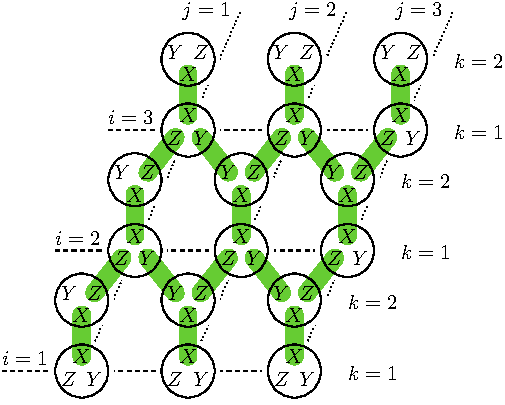
\includegraphics[width=0.6\columnwidth]{fig_00.pdf}
\caption{
Gauge generators have support on the edges of the honeycomb lattice.
Qubits here are depicted as circles.
}
\label{honeycomb}
\end{center}
\end{figure*}


The Kitaev honeycomb model \cite{Kitaev2006} is built from spins on
the sites of a hexagonal lattice. 
The lattice of linear size $l$ has $n=2l^2$ sites
which we coordinatize using integer triples $i, j, k$
with $1\le j, k\le l$ and $k=1, 2.$
We use periodic boundary conditions so $i, j$ are
to be taken modulo $l$.
See figure \ref{honeycomb}.
The edges of the lattice are in one-to-one
correspondence with the generators $G_0$:
$$
G_0 := \big\{X_{ij1}X_{ij2},\ Z_{ij2}Z_{i+1,j1},\ Y_{ij1}Y_{i-1,j+1,2}
\ \mbox{for}\ 1\le i,j\le l\big\}.
$$
Note that we make the definition $Y:=XZ$ for each site.

Stabilizers are generated from closed strings of
gauge operators. 
For example, each hexagon gives a stabilizer
\begin{align*}
h_{ij}:&= 
X_{ij1}X_{ij2}
Z_{ij2}Z_{i+1,j1}
Y_{i+1,j1}Y_{i,j+1,2}
X_{i,j+1,2}X_{i,j+1,1}
Z_{i,j+1,1}Z_{i-1,j+1,2}
Y_{i-1,j+1,2}Y_{ij1}
\\
&= 
Z_{ij1} Y_{ij2} X_{i+1,j1}
Z_{i,j+1,2} Y_{i,j+1,1} X_{i-1,j+1,2}.
\end{align*}

And the two homologically non-trivial loops
give stabilizers:
$$
h_v := \prod_{i=1}^l Y_{i11} Y_{i12},\ \ 
h_h := \prod_{j=1}^l X_{1j2} X_{2j1}.
$$

This gives independant stabilizer generators $\Stab_0$
from each hexagon, less one, as well as $h_v$ and $h_h.$
%two homologically non-trivial loops.
The number of hexagons is $\frac{1}{2}n$ and
so we find $|\Stab_0|=\half n+1.$
There are no logical operators, so we
must have $|R_0|=n-2.$

\begin{figure*}[th!]
\begin{center}
        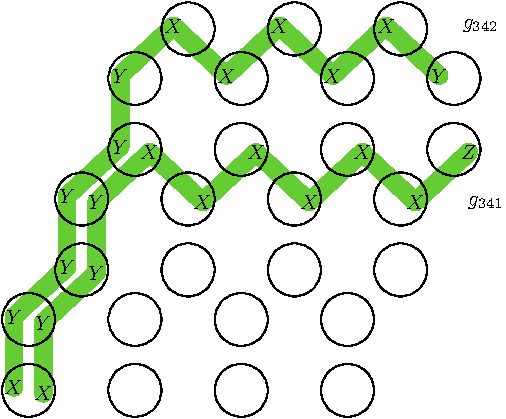
\includegraphics[width=0.5\columnwidth]{fig_01.pdf}
%\caption{Two elements $g_{341}$ and $g_{342}$ of the set $R_0$}
\caption{Two elements of the set $R_0$ corresponding
to $i=3$, $j=4$ and $k=1,2.$}
\label{jaws}
\end{center}
\end{figure*}

Now we construct a set of string operators $R_0$,
one for each site on the lattice, except for
the two sites $(1,1,1)$ and $(1,1,2).$
Each string $g_{ijk}\in R_0$
is constructed as the product of
gauge operators along a path starting at
$(1,1,1)$ and terminating at $(i,j,k).$
See figure \ref{jaws}.
Each such path is built from two ``straight''
path segments, first in the $i$ direction
and then in the $j$ direction. 
The paths for operators $g_{ij1}$ and
$g_{ij2}$ coincide along the $i$ direction
but become disjoint in the $j$ direction:
the $g_{ij1}$ path goes around the bottom
of the hexagons and the $g_{ij2}$ path
goes around the top.
%In \cite{Kells2009} they introduce a set of
%mutually anti-commuting string operators $R_0.$
With periodic boundary conditions $R_0$ forms an
independant generating set of $R$ of size $n-2.$

We construct an isomorphism $\phi: R\to \Pauli_r$
by sending elements of $R_0$ bijectively
to the following independant generating
set of $\Pauli_r$:
$$
\big\{c_{2j}:=Z_1...Z_{j-1} X_j,\ c_{2j+1}:=Z_1...Z_{j-1} Y_j\ \ \mbox{for}\ 1\le j\le r\big\}.
$$
The bijection is constrained 
by setting $\phi(g_{ij1}):=c_{2j'+1}$
and $\phi(g_{ij2}):=c_{2j'}$
where $j'$ is chosen uniquely for each $i, j.$
The $c_j$ are paired Majorana fermion operators \cite{Kitaev2006}.

%We construct an isomorphism $\phi: R\to \Pauli_r$
%by setting $\phi(g_{ij1}):=c_{2j'}$
%and $\phi(g_{ij2}):=c_{2j'+1}$
%%we map 
%%elements of $R_0$ to the following independant generating
%where the $c_j$ form the following independant generating
%set of $\Pauli_r$:
%$$
%%\big\{\prod_{i=1}^{j-1} Z_i X_j,\ \prod_{i=1}^{j-1} Z_i Y_j\ \mbox{for}\ 1\le j\le r\big\}.
%\big\{c_{2j}:=Z_1...Z_{j-1} X_j,\ c_{2j+1}:=Z_1...Z_{j-1} Y_j\ \ \mbox{for}\ 1\le j\le r\big\}.
%$$

We check this is a group homomorphism by showing that relations
satisfied by elements of $R_0$ are satisfied by
their images under $\phi.$
All such relations are either of the form
$g^2=~\pm~I$, $gg'=\pm~g'g$, or
products thereof.
So it is sufficient to check squares of
elements and commutation relations.
Every element of $R_0$ anticommutes with
every other element of $R_0$, and this is true also
of the $c_j.$
Also, $g_{ij1}^2=-I$ and $g_{ij2}^2=I$ 
is preserved by $\phi$ because $c_{2j}^2=I$ and $c_{2j+1}^2=-I$.
Finally, $\phi$ is an isomorphism
because it is a bijection of two independant
generating sets.

The next step is to write each element of $G_0$
as a product of reduced gauge operators and stabilizers.
The key thing to note is that the product of two
operators $g_{ijk}, g_{i'j'k'}\in R_0$ gives a string
operator between the sites $(i,j,k)$ and $(i',j',k')$.
And {\it any} string operator between these
two sites can then be generated by using stabilizers to
``deform'' the string $g_{ijk}g_{i'j'k'}.$
For example, taking the product
of two operators from $R_0$ that differ
by one path segment gives the following:
\begin{align*}
Z_{ij2}Z_{i+1,j,1} &= g_{ij2} g_{i+1,j,1} \\
%&\mbox{for}\ \  1\le i<l,\ 1\le j\le l, \ \ \mbox{except}\ \  (i,j)=(1,1) \ \ \mbox{or}\ \ (l,1)\\
Y_{i+1,j,1}Y_{i,j+1,2} &= g_{i+1,j,1}g_{i,j+1,2}
%&\mbox{for}\ \  1\le i,j\le l, \ \ \mbox{except}\ \  (i,j)=(1,1) \ \ \mbox{or}\ \ (l,1).
\end{align*}
We need the homologically non-trivial stabilizers to get these:
\begin{align*}
Z_{lj2}Z_{1j1} &= h_v g_{lj2} g_{1j1} &\mbox{for}\ \  2\le j\le l
\end{align*}
And the $X_{ij1}X_{ij2}$
gauge operators can be generated
by the product of 
$g_{ij1}g_{ij2}$ and the enclosed hexagon stabilizers:
$$X_{ij1}X_{ij2}=g_{ij1}g_{ij2}\prod_{j'=1}^{j-1} h_{ij'}.$$

The only $G_0$ operators that are not 
quadratic in $R_0$ operators are the five
operators that touch either of the sites
$(1,1,1)$ or $(1,1,2)$.

So each block in the Hamiltonian
is seen to be quadratic in the $c_j$ plus
five other Pauli operator terms which we denote as $\Lambda_\rho$:
$$
    \Ham_\rho = \sum_{ij} \Gamma_{ij}(\rho) c_i c_j + \Lambda_\rho
$$
The coefficients $\Gamma_{ij}$ are dependant on the irrep $\rho.$

%A similar analysis applies to the ising model, Jordan-Wigner... 
%http://arxiv.org/pdf/1504.01444 page 86.

%%%%%%%%%%%%%%%%%%%%%%%%%%%%%%%%%%%%%%%%%%%%%%%%%%%%%%%%%%%%%%%%%%%%%%%%%%%%%%%
%
%%%%%%%%%%%%%%%%%%%%%%%%%%%%%%%%%%%%%%%%%%%%%%%%%%%%%%%%%%%%%%%%%%%%%%%%%%%%%%%
%

%\subsection{Self-representations}
%
%In general we can represent $G=\Stab\times R$ in $R$ itself..
%and if we construct generators $R_0$ of $R$ by discarding
%elements of $G$ (ie. $R_0\subset G$), then the resulting
%Hamiltonian blocks look like a smaller version
%of the original code, along with ``frozen'' logical
%operators and stabilizers. {\it XXX work all this out XXX}


%%%%%%%%%%%%%%%%%%%%%%%%%%%%%%%%%%%%%%%%%%%%%%%%%%%%%%%%%%%%%%%%%%%%%%%%%%%%%%%
%
%%%%%%%%%%%%%%%%%%%%%%%%%%%%%%%%%%%%%%%%%%%%%%%%%%%%%%%%%%%%%%%%%%%%%%%%%%%%%%%
%

\appendix
\section{Character theory}
\label{appendix}

Given a group representation $\rho:G\to GL(V)$
the {\it character} of $\rho$ is a function
$\chi_\rho:G\to \Complex$ given by
$$
    \chi_\rho(g) = \mbox{Tr}\ \rho(g).
$$

Given two functions $u,v : G \to \Complex$ 
we define the following inner product:
$$
    \langle u, v \rangle := \frac{1}{|G|} \sum_{g\in G} u(g) \overline{v(g)}.
$$

The character of the Pauli representation, $\chi_{{pauli}}:\Pauli_n\to\Complex$
is given by:
$$
\chi_{{pauli}}(g) = \sum_{v \in basis} \langle v | \rho_{{pauli}}(g) | v \rangle
    = \left\{ \begin{array}{ll}
 \pm 2^n &\mbox{if}\ g=\pm I\\
 0 &\mbox{otherwise}\end{array}\right.
$$

Since $|P_n|=2^{2n+1}$ it follows that
$\langle\chi_{pauli},\chi_{pauli}\rangle = 1$ and
so $\rho_{pauli}$ is an irreducible representation of $\Pauli_n.$

For $G$ a subgroup of $\Pauli_n$, and decomposition
into a direct product $G=\Stab\times \Pauli_r$ we have the
following representations:
$$
    \rho(g) = \rho_1(h) \rho_{pauli}(g'),
$$
where $g=hg'$, $h\in \Stab$, $g'\in \Pauli_r$ and $\rho_1(h)$ is
a $1$-dimensional representation of $\Stab$.
And $\rho_{pauli}$ here is the $2^r$ dimensional Pauli representation.
The character for this representation is:
$$
\chi_{{\rho}}(hg') = \rho_1(h) \sum_{v \in basis} \langle v | \rho_{{pauli}}(g') | v \rangle
    = \left\{ \begin{array}{ll}
 \pm 2^r\rho_1(h) &\mbox{if}\ g'=\pm I\\
 0 &\mbox{otherwise}\end{array}\right.
$$

Once again, $|G|=2^{2r+m+1}$ and so
$\langle\chi_{\rho},\chi_{\rho}\rangle = 1$ and
$\rho_{\rho}$ is an irreducible representation of $G.$
We now count the occurances of 
this representation in $\rho_{pauli}$:
\begin{align*}
\langle\chi_{pauli},\chi_{\rho}\rangle &= \frac{1}{|G|}\sum_{g\in G} \chi_{pauli}(g)\overline{\chi_{\rho}(g)} \\
&= \frac{1}{2^{2r+m+1}} \sum_{g=\pm I} 2^n 2^r = \frac{2^{n+1+r}}{2^{2r+m+1}} = 2^k
\end{align*}
where $k$ is the number of logical qubits so that $n=r+m+k.$

\bibliography{refs}{}
\bibliographystyle{abbrv}


\end{document}


